\documentclass[twocolumn,letterpaper,spanish]{revtex4}
%%%%%%%%%%%%%%%%%%%%%%%%%%%%%%%%%%%%%%%%%%%%%%%%%%%%%%%%%%%%%%%%%%%%%%%%%%%%%%%%%%%%%%%%%%%%%%%%%%%%%%%%%%%%%%%%%%%%%%%%%%%%
\usepackage{amsmath}
\usepackage{epsfig}
\usepackage{bm}
%\usepackage[spanish]{babel}
\usepackage{graphicx}
\usepackage{amsmath}
\usepackage{cancel}
\usepackage{subfig}
\usepackage{amsmath}
\numberwithin{equation}{section}
\DeclareMathOperator{\arcsinh}{arcsinh}
\DeclareMathOperator{\arccosh}{arccosh}
\renewcommand\thesection{\arabic{section}}
\renewcommand\thesubsection{\thesection.\arabic{subsection}}
\usepackage[spanish,es-tabla]{babel}
\usepackage{caption}


\newcommand{\be}{\begin{equation}}
\newcommand{\ee}{\end{equation}}
\newcommand{\beq}{\begin{eqnarray}}
%\newcommand{\tcancel}[1]{\leavevmode\cancel{#1}}
\spanishdecimal{.}

\begin{document}

\title{Mapa del Fondo Cósmico de Microondas}
\author{Constanza Osses Guerra}
\email{conyosses@gmail.com}
\affiliation{Profesor: Crist\'obal Sif\'on}
\affiliation{Doctorado en Ciencias F\'isicas, Pontificia Universidad Cat\'olica de Valpara\'{\i}so, Chile}

\begin{abstract}
 Este trabajo tiene por objetivo recrear el mapa del CMB a partir de un espectro de potencias dado. En la primera sección se pretende obtener dicho mapa, en la segunda secci\'on obtener el espectro de potencias a partir del mapa generado anteriormente, y finalmente, se obtendr\'an los valores de los par\'ametros $\Omega_b h^2$ y $\Omega_c h^2$ utilizados para generar el espectro de potencias original.
\end{abstract}


\maketitle
\section{Introducción}

El estudio del Fondo C\'osmico de Microondas (CMB) \cite{cmb} ha otorgado la oportunidad de conocer m\'as a fondo el Universo. A trav\'es del CMB se pueden estudiar diferentes \'areas de la cosmolog\'ia como ondas gravitacionales primordiales, propiedades de los neitrinos y distribuciones de masas.

Adem\'as el CMB nos proporciona la mejor evidencia que respalda la teor\'ia del Big Bang debido a su gran uniformidad y sus peque\~nas anisotrop\'ias. 

Por otro lado, el CMB est\'a polarizado en dos tipos: modos E y modos B. El modo E surge de la dispersi\'on de Thomson en el plasma mientras que el modo B puede surgir tanto de lentes gravitacionales producidos por los modos E como de ondas gravitacionales primordiales.

Diversos experimentos se han realizado con el objetivo de mejorar las mediciones del CMB tales como COBE \cite{cobe}, WMAP \cite{wmap}, Planck \cite{planck}, ACT \cite{act}, SPT y BICEP/Keck Array \cite{bicep}.

Del espectro de potencias del CMB se puede extraer mucha informaci\'on: 
De su espectro de potencias, se puede obtener informaci\'on valiosa: a peque\~nas escalas se puden apreciar fluctuaciones generadas por Inflaci\'on,  adem\'as, sus peak entregan informaci\'on sobre curvatura (primer peak), cantidad de materia bari\'onica (segundo peak) y materia oscura (tercer peak). Por otro lado, el mapa del CMB entrega informaci\'on sobre su temperatura  y c\'omo es el patr\'on de las fluctuaciones.

En este trabajo se pretende recrear un mapa del CMB y obtener los par\'ametros de densidad que generaron el espectro de potencias. En §\ref{datos} se describen los datos utilizados, en §\ref{analisis} se describe el procedimiento utilizado para llevar a cabo los objetivos, en §\ref{resultados} se exponen los resultados obtenidos y finalmente se concluye con una discusi\'on en §\ref{discusion}.

\section{Datos}\label{datos}

Los datos utilizados provienen del \textit{Code for Anisotropies in the Microwave Background (CAMB)} que est\'a basado en el CMBFast \citep{cmbfast}. Este c\'odigo es usado para calcular los espectros de potencias de temperatura y polariazaci\'on del CMB, espectros angulares, funciones de transferencia entre otros.

 En este c\'odigo existen diferentes componentes del espectro de potencias: total, unlensed\_scalar, unlensed\_total, lensed\_scalar, tensor, lens\_potential. Trabajaremos s\'olo con la componente unlensed\_scalar.

El espectro de potencias se origina con ciertos par\'ametros iniciales, de los cuales debemos identificar los valores de los par\'ametros de densidad bari\'onica ($\Omega_b\,h^2$) y de materia oscura ($\Omega_c\,h^2$)

\section{An\'alisis}\label{analisis}

La amplitud de las fluctuaciones del espectro de potencias est\'a relacionada con los arm\'onicos esf\'ericos y est\'a dada por


\begin{equation}
C_{\ell} = \frac{1}{2\ell+1}\sum_{m =-\ell}^{\ell}\langle \,|a_{\ell m}|^2\,\rangle
\end{equation}

\subsection{Mapa CMB}\label{mapa}

Queremos obtener el mapa del CMB en 2D, para ello, primero debemos obtener el mapa en espacio real a partir de los datos entregados por el espectro original.
A partir de los datos entregados del espectro original, se puede obtener una grilla 
\begin{equation}
\tilde{\mathbf{M}}(\ell_x,\ell_y)=C\left(\sqrt{\ell_x^2 + \ell_y^2}\right)
\end{equation}
donde $\ell=\sqrt{\ell_x^2 + \ell_y^2}$

Para cada par de datos de $\ell_x, \ell_y$ se obtiene un valor asociado dado por el espectro de potencias original.

Se debe ir rellenando la grilla con los correspondientes valores de $C(\sqrt{\ell_x^2 + \ell_y^2})$. Se debe tomar en cuenta que los valores entregados para cada momento multipolar corresponden a una cantidad $D_{\ell}$ multiplicada por un factor, entonces

\begin{equation}
C_{\ell} = \frac{2\pi\,D_{\ell}}{\ell\,(\ell+1)}
\end{equation}

Esta funci\'on nos otorga el mapa del CMB para el espacio real.

Como el espectro de potencias se genera de fluctuaciones primordiales de tipo gaussiana, es necesario introducir una funci\'on de distribuci\'on gaussiana al espectro final en el espacio de Fourier, de tal manera que

\begin{equation}
\mathbf{M}\left(\theta_{x}, \theta_{y}\right)=\int d \ell_{x} \int d \ell_{y} \exp \,[-2 i(\vec{\ell} \cdot \vec{\theta})] \,\tilde{\mathbf{M}}\left(\ell_{x}, \ell_{y}\right)\, \tilde{\mathbf{G}}\left(\ell_{x}, \ell_{y}\right)
\end{equation}

donde 
\begin{equation}
\tilde{\mathbf{G}}\left(\ell_{x}, \ell_{y}\right)=\int d \ell_{x} \int d \ell_{y} \,\exp\, [-2 i(\vec{\ell} \cdot \vec{\theta})] \,\mathcal{N}(\mu, \sigma)
\end{equation}

Se debe tener en cuenta que los momentos multipolares se relacionan con el \'angulo en el cielo de la siguiente manera: $\ell=\frac{2\pi}{\theta}$

\subsection{Espectro de Potencias}\label{espectro}

Como existen problemas de discontinuidad en los bordes del mapa generado en la secci\'on anterior, es necesario apodizarlo, es decir, multiplicarlo con una funci\'on ventana. Para contrarrestar el efecto de los bordes, esta funci\'on debe decaer a cero suavemente. 

\begin{equation}
\mathbf{M}_{\text {apod }}\left(\theta_{x}, \theta_{y}\right)=\mathbf{M}\left(\theta_{x}, \theta_{y}\right) \circ \mathbf{W}\left(\theta_{x}, \theta_{y}\right)
\end{equation}
donde $\circ$ es el producto de Hadamard.

Una vez obtenido el mapa apodizado, se procede a calcular el mapa en espacio real, de tal forma que
\begin{equation}
\tilde{\mathbf{M}}\left(\ell_{x}, \ell_{y}\right)=\operatorname{FFT}\left(\mathbf{M}_{\text {apod }}\left(\theta_{x}, \theta_{y}\right)\right)
\end{equation}

Con este mapa se pueden ir calculando los coeficientes $C_\ell$ del espectro, de modo que se promedie para cada anillo con momento multipolar constante y se eleve al cuadrado 

\begin{equation}
C_{\ell}\left(\sqrt{\ell_{x}^{2}+\ell_{y}^{2}}\right)=\left\langle\tilde{\mathbf{M}}\left(\ell_{x}, \ell_{y}\right)\right\rangle
\end{equation}

Se debe tener en cuenta la relaci\'on entre $D_{\ell}$ y $C_{\ell}$ dada por la ec. (3.2).

Si bien esta ecuaci\'on nos entregar\'a un espectro de potencias, se debe corregir debido a algunos errores que son causados por la apodizaci\'on. Estos errores se corrigen mediante la siguiente ecuaci\'on

\begin{equation}
\hat{D}_{\ell}=T_{\ell} * D_{\ell}+N_{\ell}
\end{equation}
donde $\hat{D}_{\ell}$ es el espectro a partir del mapa, $D_{\ell}$ es el espectro real, $T_{\ell}$ es la funci\'on de transferencia, y $N_{\ell}$ es el sesgo de ruido.
Por lo tanto, se puede construir el espectro de potencias real obteniendo los valores de la siguiente manera
\begin{equation}
D_{\ell}=\frac{\left(\hat{D}_{\ell}-N_{\ell}\right)}{T_{\ell}}
\end{equation}


\subsection{Par\'ametros de densidad}\label{parametros}

Para obtener un espectro igual o similiar al espectro original, se debe iterar sobre los par\'ametros de densidad del paquete otorgado por CAMB. Teniendo los datos para cada espectro generado, se puede calcular una prueba de independencia entre las distribuciones a trav\'es de $\chi^2$

\begin{equation}
\chi^2 = \displaystyle\sum_{i} \frac{(x_{i,obs} - x_{i,teo})^2}{x_{i,teo}}
\end{equation}

donde $x_{obs}$ es el valor de un punto en el espectro observado y $x_{teo}$ es el valor de un punto en el espectro original.

Este test indica que mientras menor sea el valor $\chi^2$, existe una mayor probabilidad de que ambas distribuciones sean iguales. Es decir, para obtener los valores de los par\'ametros de densidad es necesario que el valor de $\chi^2$ normalizado por los grados de libertad (dof = n\'umero de datos - par\'ametros libres - 1) al comparar el espectro resultante con el otriginal, sea lo m\'as cercano a cero posible.


\section{Resultados}\label{resultados}

Los datos entregados generan el siguiente espectro de potencias

\begin{center}
   \includegraphics[width=85mm]{spectrum_original2.png}\\
   Figura 1.\emph{\ Espectro de potencias original.}
\end{center}
donde los momentos multipolares var\'ian entre $2\leq\ell\leq 5049$. Tanto el momento monopolar ($\ell=0$) como el dipolar ($\ell=1$) no contribuyen al espectro. El monopolo no contribuye porque representa el promedio de las fluctuaciones de temperatura en el cielo y asumiendo homogeneidad e isotrop\'ia debe ser cero, mientras que el dipolo es afectado por el propio movimiento de la Tierra, viendose el background corrido hacia el rojo en un sector y hacia el azul en el lado opuesto. Entonces, para mayor precisi\'on en los c\'alculos se opta por remover estos dos t\'erminos de los momentos dipolares.


\subsection{Mapa CMB}

De los datos del espectro original, tomamos la columna $D_{\ell}$, la transformamos en $C_{\ell}$ de acuerdo a la ec. (3.2) e iteramos dos veces sobre un rango determinado para formar la matriz en 2 dimensiones. El rango m\'aximo de los elementos de la iteraci\'on est\'a dictaminado por la resoluci\'on de nuestro mapa. En este caso, la resoluci\'on es de 7' lo cual nos entrega $\ell_{max}=3086$. Se debe tener en cuenta que el valor m\'aximo de $\ell$ es 5049, por lo que si el m\'odulo de las dos variables es mayor, el elemento correspondiente de la matriz es cero. El mapa en espacio real se puede apreciar en la Fig. 2. En \'el, podemos ver anilos con un cierto valor constante de $C_{\ell}$ el cual va disminuyendo a medida que aumentan los momentos multipolares.
Se debe destacar adem\'as, que el primer anillo comienza en $\ell\sim 100-125$, lo cual coincide bastante bien con el primer peak del espectro original.

\begin{center}
   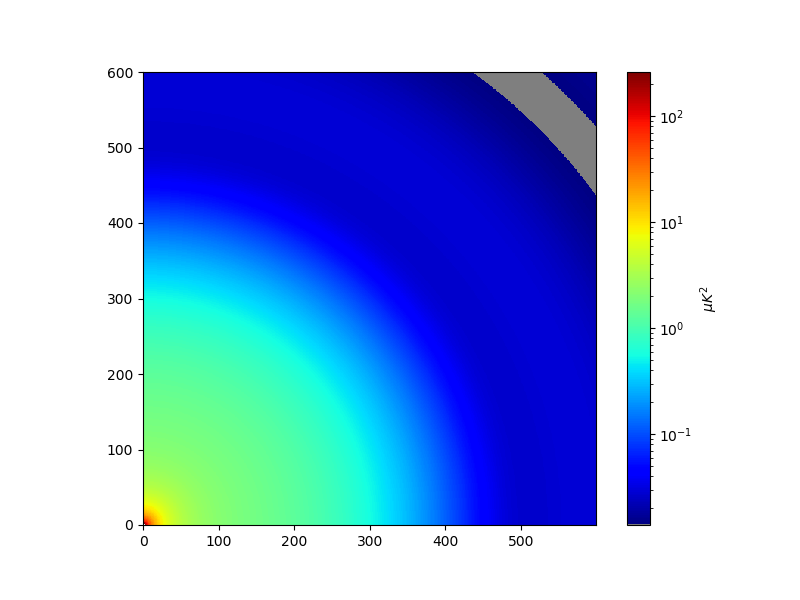
\includegraphics[width=85mm]{M_tilde.png}\\
   Figura 2.\emph{\ Mapa en espacio real $(\tilde{\mathbf{M}}(\ell_x, \ell_y))$. Los valores de $C_{\ell}$ disminuyen mientras los valores de $\ell_x$ y $\ell_y$ aumentan. El primer anillo naranja corresponde al primer peak del espectro de potencias.}
\end{center}

Asumiendo Gaussianeidad y de acuerdo a la ec. (3.4) tomamos la Transformada R\'apida de Fourier (inversa) en 2-dimensiones de una distribuci\'on Gaussiana (en este caso, una distribuci\'on normal con $\mu=0$, $\sigma=1$) de la misma longitud que la matriz $\tilde{\mathbf{M}}(\ell_x, \ell_y)$ creada anteriormente. Tomando la parte real de $\tilde{\mathbf{G}}(\ell_x \ell_y)$ obtenemos el siguiente mapa

\begin{center}
   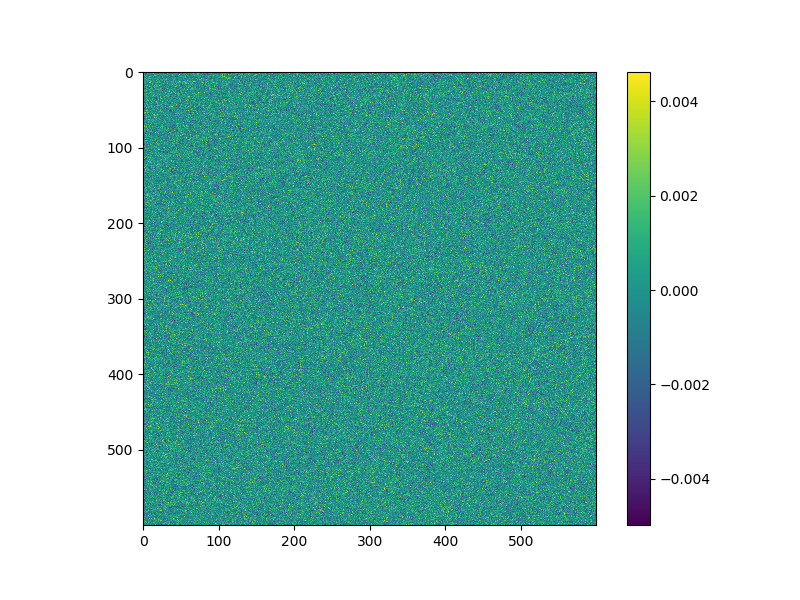
\includegraphics[width=85mm]{G_ell.png}\\
   Figura 3.\emph{\ Transformada de Fourier en 2 dimensiones (FFT) de una distribuci\'on normal con $\mu=0$ y $\sigma=1$.}
\end{center}

Una vez obtenidos $\tilde{\mathbf{M}}(\ell_x, \ell_y)$ y $\tilde{\mathbf{G}}(\ell_x, \ell_y)$ podemos usar la ec. (3.3) para obtener el mapa del CMB en espacio de Fourier

\begin{center}
   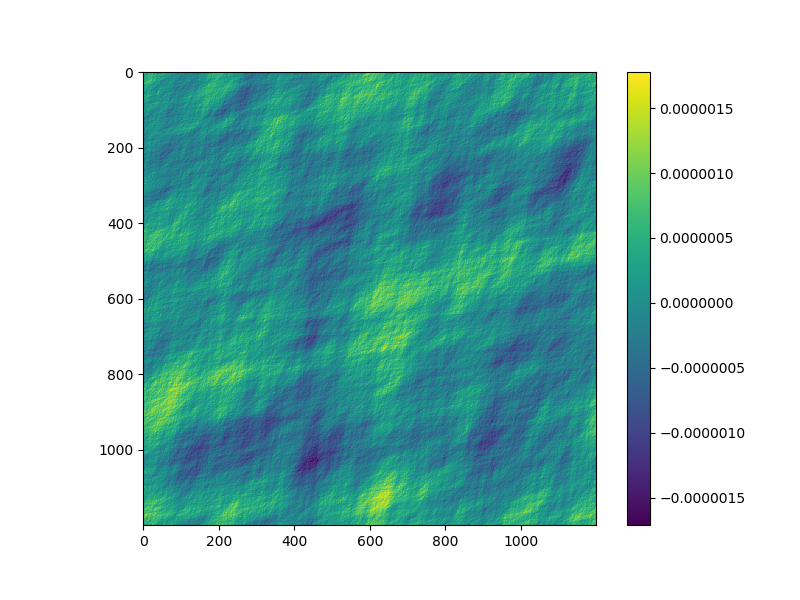
\includegraphics[width=85mm]{M_tetha.png}\\
   Figura 4.\emph{\ Mapa del CMB en espacio de Fourier.}
\end{center}

Al reescalar el mapa para convertir los ejes en grados y la temperatura del orden de $10^2$, se obtiene un mapa del mismo color en todos los sectores

\begin{center}
   \includegraphics[width=85mm]{M_tetha-2.png}\\
   Figura 5.\emph{\ Mapa del CMB en espacio de Fourier reescalado a grados.}
\end{center}

\subsection{Espectro de Potencias}

Ahora queremos obtener el espectro de potencias a partir del mapa anterior. Para ello, primero se debe escoger una funci\'on ventana que no decaiga muy r\'apido a cero. En este trabajo, se escogi\'o la funci\'on ventana de Hann.

\begin{center}
   \includegraphics[width=85mm]{window.png}\\
   Figura 6.\emph{\ Funci\'on ventana de Hann.}
\end{center}

Entonces, el mapa apodizado queda de la siguiente manera

\begin{center}
  \includegraphics[width=85mm]{M2_ell.png}\\
   Figura 7.\emph{\ Mapa del CMB apodizado.}
\end{center}

El mapa apodizado a partir del mapa reescalado queda de la siguiente manera

\begin{center}
  \includegraphics[width=85mm]{M2_ell-2.png}\\
   Figura 8.\emph{\ Mapa del CMB apodizado y reescalado.}
\end{center}


Calculando para cada anillo el promedio de la transformada de Fourier del mapa apodizado se obtiene el valor del coeficiente $C_{\ell}$ y usando la ec. (3.2) se encuentran los valores $D_{\ell}$ del espectro de potencias.


Para corregir los errores de la apodizaci\'on y resoluci\'on del mapa se debe introducir el sesgo de ruido (se utiliz\'o una distribuci\'on normal) y una funci\'on de transferencia. El gr\'afico del espectro sin corregir queda de la siguiente manera 

\begin{center}
  \includegraphics[width=85mm]{D2_ell.png}\\
   Figura 9.\emph{\ Mapa del CMB apodizado y reescalado.}
\end{center}

Si bien no se logr\'o obtener la curva del espectro de potencias, se pudo calcular la diferencia entre los coeficientes del espectro nuevo con el sesgo de ruido, resultando en el siguiento gr\'afico

\begin{center}
   \includegraphics[width=85mm]{resta.png}\\
   Figura 10.\emph{\ Diferencia para el total de los coeficientes del nuevo espectro y el sesgo de ruido.}
\end{center}


\begin{center}
   \includegraphics[width=85mm]{dif.png}\\
   Figura 11.\emph{\ Diferencia iternado para cada uno de los coeficientes del nuevo espectro y el sesgo de ruido.}
\end{center}


\subsection{Par\'ametros de densidad}

Para obtener los espectros, s\'olo se modificaron los par\'ametros de densidad biri\'onica y de materia oscura. Los dem\'as par\'ametros se dejaron tal cual estaban en el paquete entregado por CAMB y son los siguientes 

\begin{center}
\begin{tabular}{c | c}
	\,Par\'ametro\, & \,Valor\, \\ \hline
	$A_s$\,  &  \,2$\times10^{-9}$ \\
	$n_s$\,  &  0.965 \\
 	$r$\,    &  0.00  \\
 	$H_0\,(km\,s^{-1}\,Mpc^{-1})$\, &  67.5 \\
 	$\sum m_{\nu}\,(eV)$ & 0.06 \\ 
 	$\Omega_k$ & 0.00 \\
 	$\tau$  & 0.06 \\ 
\end{tabular}\label{tabla1}
\captionof{table}{Par\'ametros iniciales entregados por CAMB}
\end{center}

Usando estos valores y el c\'odigo de CAMB en Python, se iter\'o en primera instancia 10 veces sobre cada par\'amtro $\Omega_b h^2$ y $\Omega_b h^2$, entre 0.005 y 0.150. Se compar\'o cada espectro resultante con el original, obtenieno un valor de $\chi^2$ que posteriormente es normalizado por los grados de libertad (dof = 5046). La Tabla 1 muestra los mejores valores de $\Omega_b h^2$, $\Omega_b h^2$ con $\chi^2<100000$. 

\begin{center}
\begin{tabular}{| c | c | c | c |}\hline
$\Omega_b h^2$ & $\Omega_c h^2$ & $\chi^2$ & $\chi^2/$grados de libertad    \\ \hline
	\,0.0533  & \,0.0694\,  &  \,90448.6914\,  &  17.9248 \\
	0.0533  & 0.0856  &  19162.9253  &  3.7976 \\
	0.0533  & 0.1017  &  27735.4469  &  5.4965 \\
	0.0533  & 0.1178  &  75457.1964  & 14.9539 \\
	0.0694  & 0.1017  &  55901.4234  & 11.0784 \\
	0.0694  & 0.1178  &  30447.5212  &  6.0339 \\
	0.0694  & 0.1339  &  35793.6990  &  7.0935 \\
	0.0694  & 0.1500  &  58884.4855  & 11.6695 \\ \hline
\end{tabular}\label{tabla1}
\captionof{table}{Mejores resultados de $\chi^2$ para las primeras 11 iteraciones:$0.05<\Omega_b h^2$, $\Omega_b h^2<0.150$. En la primera columna se muestran los valores del par\'ametro de densidad bari\'onica $\Omega_b h^2$, en la segunda columna, el par\'ametro de densidad de materia oscura $\Omega_c h^2$, la tercera columna corresponde a los valores de $\chi^2$ y en la cuarta columna se muestran los valores de $\chi^2$ normalizados por los grados de libertad. El mejor resultado del test ($\chi^2/dof = 3.7976$) corresponde a $\Omega_b h^2=0.0533$ y $\Omega_c h^2=0.0856$.}
\end{center}

Posteriormente, se realiz\'o el mismo procedimiento, escogiendo ahora un rango de los par\'ametros cercanos a los valores que entregaban resultados m\'as bajos de $\chi^2$, entonces, se iteraron 50 veces los par\'ametros: $0.05<\Omega_b h^2< 0.075$ y $0.05<\Omega_c h^2<0.150$. La Tabla 2 muestra los valores de los par\'ametros para valores de $\chi^2<2500$.

\begin{center}
\begin{tabular}{| c | c | c | c |}\hline
$\Omega_b h^2$ & $\Omega_c h^2$ & $\chi^2$ & \,$\chi^2/$grados de libertad\,       \\ \hline
	\,0.0592\,   & \,0.0998\, & \,2497.2344\,   & 0.4949  \\
	0.0597   & 0.1002 & 2452.5220  & 0.4860  \\
	0.0597   & 0.1006 & 2427.5886  & 0.4811  \\
	0.0597   & 0.1010 & 2436.7352  & 0.4829  \\
	0.0597   & 0.1014 & 2471.5026  & 0.4898   \\\hline
\end{tabular}\label{tabla3}
\captionof{table}{Mejores resultados para las nuevas 10 iteraciones: $0.058<\Omega_b h^2<0.064$ y $0.090<\Omega_b h^2<0.107$. El mejor valor del test es $\chi^2/dof = 0.4811$, lo cual corresponde a $\Omega_b h^2=0.0597$ y $\Omega_c h^2=0.1006$.}
\end{center}

Los dos mejores resultados expuestos en la Tabla 3 se grafican junto al espectro original en las Fig. 12 y 13. En concordacia con los resultados obtenidos a trav\'es del test $\chi^2$, el espectro que m\'as se ajusta a la curva del espectro original corresponde a los valores $\Omega_b h^2=0.0597$ y $\Omega_c h^2=0.1006$. Si bien no ajustan perfectamente porque el primer peak del espectro resultante est\'a levemente por debajo del original, mientras que en el segundo peak se ajusta bastante bien.

\begin{center}
   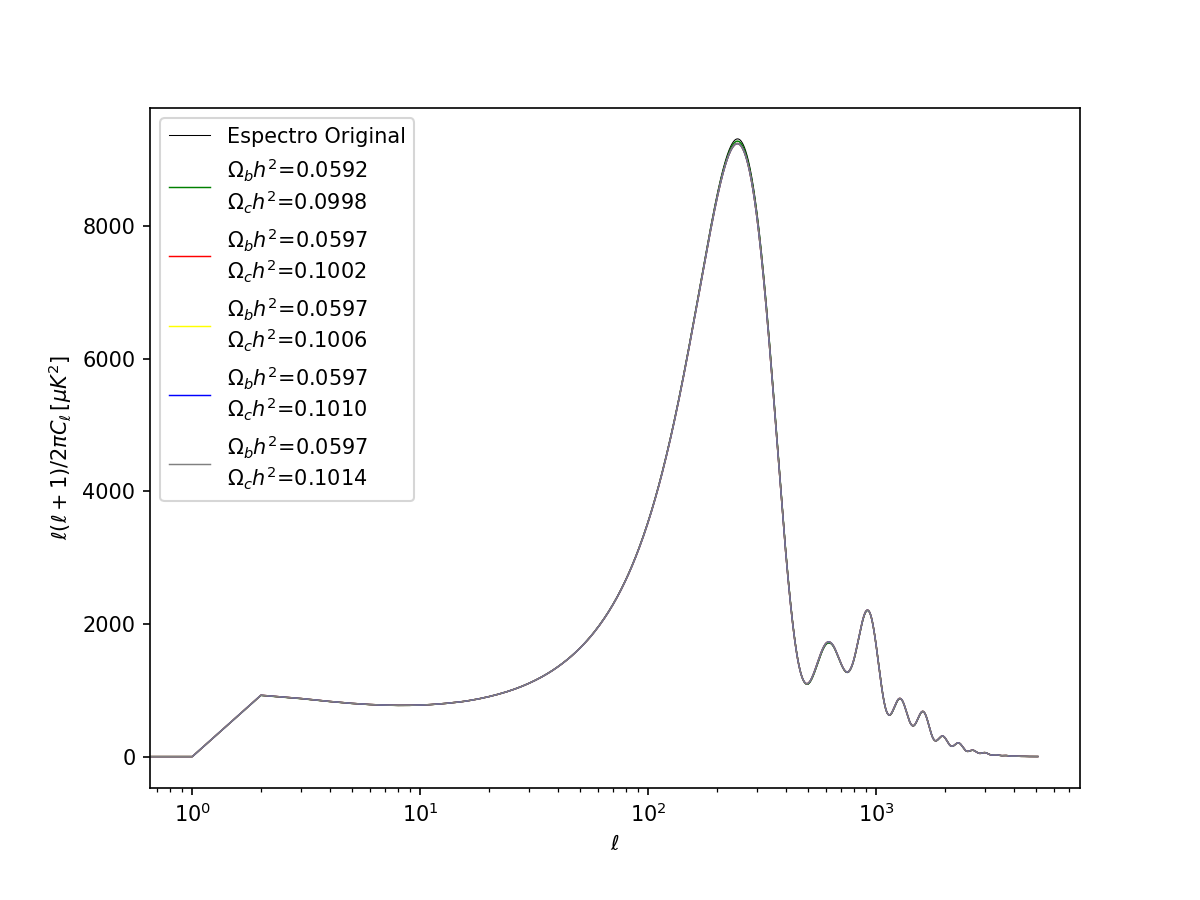
\includegraphics[width=85mm]{comparacion.png}\\
   Figura 12.\emph{\ Comparaci\'on entre los espectros obtenidos con el original. La l\'inea negra representa el espectro original mientras que las dem\'as l\'ineas representan los valores de $\chi^2<2500$.}%. Se puede observar en el gr\'afico, que la curva que m\'as se asemeja al espectro original es la verde.}
\end{center}

\begin{center}
   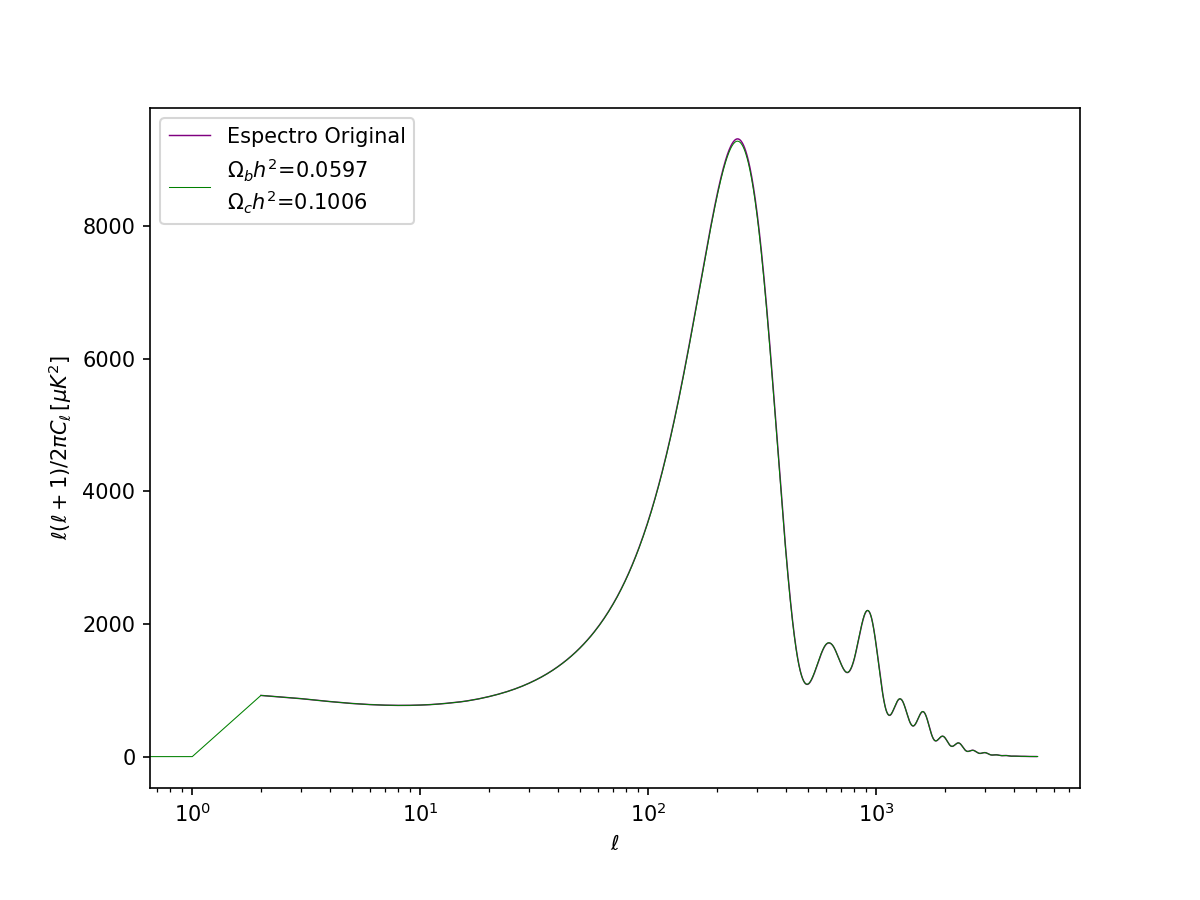
\includegraphics[width=85mm]{comparacion2.png}\\
   Figura 13.\emph{\ Comparaci\'on entre el mejor espectro obtenido con el original. La l\'inea negra representa el espectro original mientras que la l\'inea verde representa el espectro con los mejores valores para los par\'ametros: $\Omega_b h^2$=0.0597 y $\Omega_c h^2$= 0.1006.}
\end{center}



\section{Discusi\'on}\label{discusion}

Si bien el objetivo de este trabajo era recrear un mapa del CMB y posteriormente obtener su espectro de potencias, esto no ha sido del todo posible. La resoluci\'on utilizada (7') no fue la m\'as \'optima (0.5'), esto debido a problemas computacionales que no permitieron generar mayor cantidad de datos, sin embargo, en la literatura se encuentran art\'iculos que utilizan alrededor de esta resoluci\'on (\cite{comp1}, \cite{comp2}, \cite{comp3}). Con esta resoluci\'on, el mapa no quedar\'ia tan preciso y las fluctuaciones de temperatura no ser\'ian tan notorias.
En la Fig. 2 se muestra los anillos equivalentes a $\ell_x$ y $\ell_y$ constantes y el valor de $C_{\ell}$ se va haciendo cada vez menor al ir aumentando los momentos multipolares. Por otro lado, el mapa debiese estar en escala angular desde 0 a 10° y el rango de temperatura del orden de $10^2\,(\mu K)$ pero al hacer la transfromaci\'on se obtiene un mapa de un solo color (Fig. 5). Al tener este mapa errado, el c\'alculo del espectro de potencias tambi\'en lo est\'a.
Se realiz\'o el c\'alculo de los nuevos valores para $D_\ell$, sin embargo la funci\'on de transferncia no se logr\'o obtener, se trat\'o con la propia funci\'on que viene incluida en el paquete de CAMB, con la que viene por defecto en Python, pero al generar la divisi\'on de la diferencia entre los coeficientes del espectro y el sesgo con la funci\'on de transferencia, no se obtuvo resultado.


En cuanto a los valores de los par\'ametros, se pudieron obtener valores de los par\'ametros de densidad de $\Omega_b h^2 = 0.0597$ y $\Omega_c h^2 = 1.1006$ con valor de $\chi^2$ normalizado de $\chi^2/dof = 0.4811$. Si comparamos estos valores con los entregados por Planck, que son los que aparecen originalmente en el paquete de CAMB ($\Omega_b h^2 = 0.022$ y $\Omega_c h^2 = 1.122$), existe una diferencia del $\sim 17 \%$.

Finalmente, este mapa es una recreaci\'on de un mapa generado realmente por el CMB, puesto que s\'olo se tiene en consideraci\'on la parte que no involucra lentes gravitacionales, por lo que se deben considerar los modos E.







%- no pude pasar a temperatura ni grados
%- grados no concuerda
%- 10° son como l=36
%- comparar con otro trabajo
%- mapa real quetiene de diferente
%- parametros degenerados


\bibliography{referencias}

\end{document}